

\documentclass[10pt,a4paper]{article}
\usepackage[utf8]{inputenc}
\usepackage[english]{babel}
\usepackage{amsmath}
\usepackage{amsfonts}
\usepackage{amssymb}
\usepackage{graphicx}
\usepackage{caption}
\usepackage{float}
\usepackage{array}
\usepackage{booktabs}	% for horizontal lines
\usepackage{varwidth}% http://ctan.org/pkg/varwidth
\usepackage{csvsimple} % automatic table generation from csv files
\usepackage{comment}
\usepackage[style=draft, backend=biber]{biblatex}

\addbibresource{../bibliography.bib}

\title{Chapter 3 - Solution Approach DRAFT}
\author{Weber Jakob}

\begin{document}
	\maketitle
	
	\section{One dimension} \label{1D}
 	For the sake of simplicity, the following description is restricted to one dimension and B-splines as basis functions. Later, the generalization to multiple dimensions using B-splines and tensor-product splines is given. 
 
 	The goal is to model given data $$\{x_i, y_i\}, \ i = 1, ..., n$$ using a priori knowledge like monotonicity (increasing or decreasing), curvature (convex or concave), unimodality (peak or valley) or multi-modality and positivity. Using B-splines as basis functions for the estimation $\hat y =  \hat f(x_1) = X\hat \beta$ of the unknown function $y$, the least squares objective function is given by
	
	$$Q(y;\beta) = \lVert y - \hat y\rVert^2 = \lVert y - X\beta\rVert^2 $$
	
	where $X \in \mathbb{R}^{n \times k}$ is the B-spline basis for $k$ splines and $n$ data points and $\beta \in \mathbb{R}^k$ are the coefficients to be estimated. The explicit solution for the least squares objective function is given by
	
	$$\hat \beta_{LS}= (X^TX)^{-1}X^T y.$$
	
	Figure \ref{fig:smooth_bf} shows a B-spline smooth using $k=10$ splines on an equidistant grid for noisy data as well as the individual B-spline basis functions multiplied with the corresponding, estimated least squares coefficients $\hat \beta_{LS}$.
	
	\begin{figure}[H]
		\centering
		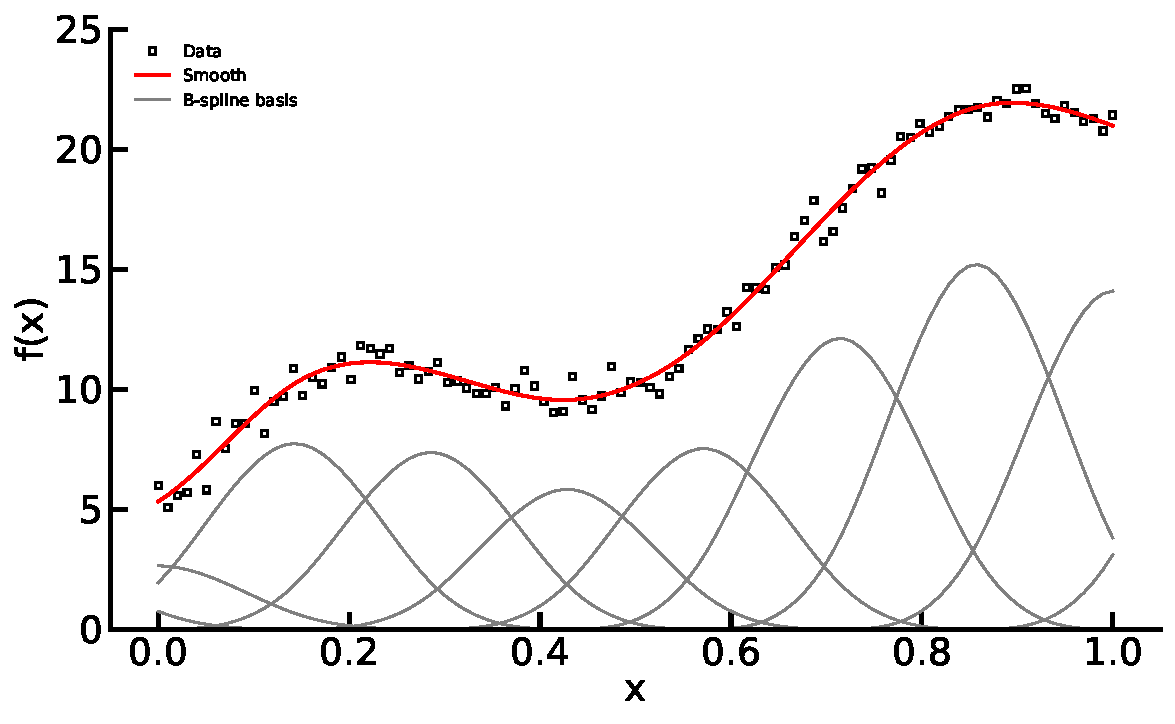
\includegraphics[width=\columnwidth]{../thesisplots/smooth_bf.pdf}
		\caption{B-spline smooth and basis functions}
		\label{fig:smooth_bf}
    \end{figure}
	
	
	The number of splines $k$ determines the amount of smoothing. Using a small number is leading to a very smooth estimate, but a large data error. On the other hand, when the number of splines is relatively large, the data error might be very small but the smoothness of the estimated function may be large. This leads to large interpolation errors and wiggle function estimates. This behavior is an example of the bias-variance dilemma and depicted in Figure \ref{fig:smooth_bf_large}. \cite{sammut2011}


	\begin{figure}[H]
	\centering
	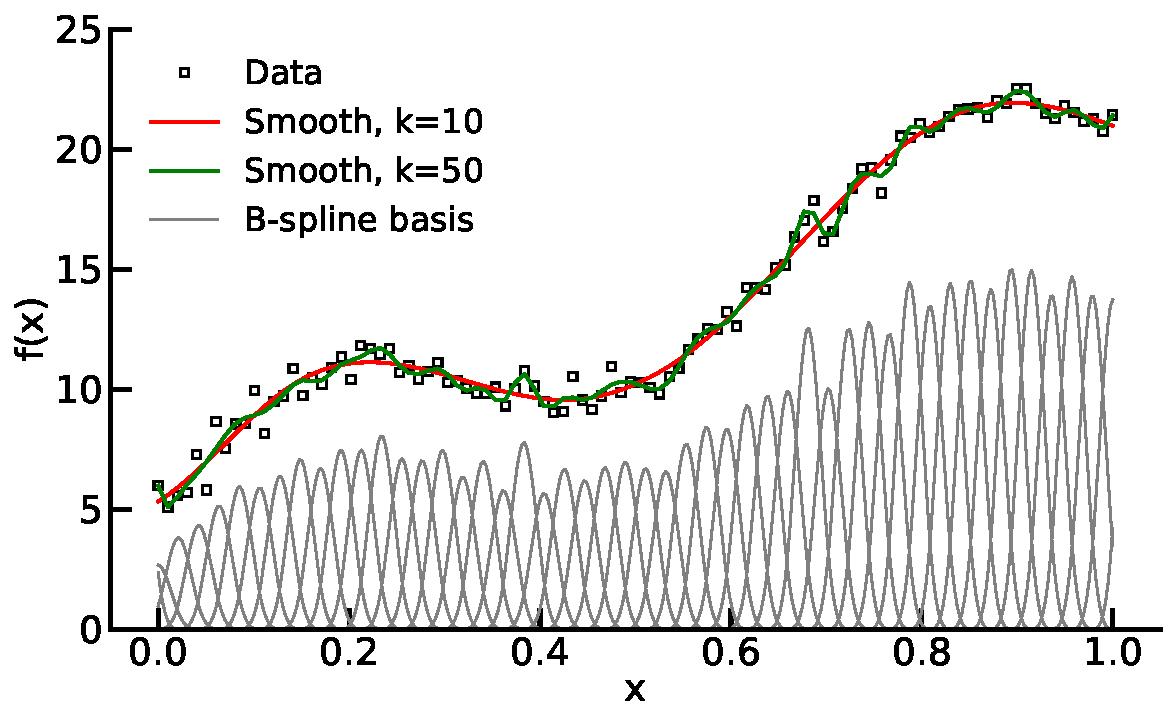
\includegraphics[width=\linewidth]{../thesisplots/smooth_wiggly_bf.pdf}
	\caption{B-spline smooth and basis functions for larger number of splines}
	\label{fig:smooth_bf_large}
	\end{figure}

	To overcome this, Eilers and Marx introduced the P-splines, which include a penalty based on the squared finite difference of order $d$ of adjacent coefficients. If $d=2$, this qualitatively  corresponds to a penalized second derivative, which itself is a measure for function wiggliness. \cite{eilers1996flexible}
	
	The difference operator $\Delta^d$ is defined by
		
	
	\begin{align*}
		\Delta^1 \beta_j &= \beta_j - \beta_{j-1} \\
		\Delta^2 \beta_j &= \Delta^1(\Delta^1 \beta_j) = \beta_j - 2\beta_{j-1} + \beta_{j-2} \\ 
	  	\vdots \\ 
	  	\Delta^d \beta_j &= \Delta^1(...(\Delta^1 \beta_j))
	\end{align*}
	
	and in matrix notation for order $d=1$
	
	$$D_1 = \begin{pmatrix} 
					-1& 1&       &        &   \\  
					  &-1& 1     &        &   \\  
					  &  &\ddots & \ddots &   \\ 
					  &  &       & -1     & 1 
			\end{pmatrix} \in R^{k-1\times k}$$
	
	and order $d=2$
	
	$$D_2 = \begin{pmatrix} 
				1& -2& 1& &    \\  
				 & 1 & -2 & 1& \\ 
				 &  & \ddots & \ddots  & \ddots \\ 
				 & & & 1 & -2 & 1 
			\end{pmatrix} \in R^{k-2\times k}$$
	
	Using the finite difference operator of order $d$, the least squares objective function is expanded to the penalized least squares objective function given by
	
	$$Q(y; \beta) = \lVert y - X\beta \rVert^2 + \lambda_s \mathcal J_s(\beta; d)$$
	
	where $\mathcal J_s(\beta; d) = \beta^T D_d^T D_d \beta$ and the smoothing parameter $\lambda_s$ determines the effect of the penalty. The matrix $D_d$ is called penalty matrix. The smoothing parameter $\lambda_s$ plays a critical role and can be optimized using the information criteria specified in Chapter Model Selection Criteria, e.g. AIC and BIC, or by using cross-validation techniques. \cite{fahrmeir2013regression}
	
	The explicit solution for the penalized least squares coefficients is then given by
	
	$$\hat \beta_{PLS} = (X^TX + \lambda_s D_d^TD_d)^{-1} X^T y.$$
	
	For small values $\lambda_s \rightarrow 0$, the penalized least squares estimate $\hat \beta_{PLS}$ approaches the least squares estimate $\hat \beta_{LS}$, while for large values $\lambda_s >> 0$, the fitted function shows the behavior of a polynomial with $d-1$ degrees of freedom. For example, using $d=2$ and a large smoothing parameter $\lambda_s$ is leading to a linear function, while using $d=1$ would lead to a constant function. \cite{fahrmeir2013regression}
	
	Figure \ref{fig:pspline} shows the behavior of P-splines using $k=50$ splines for several values of the smoothing parameter $\lambda_s = \{10^{-2}, 10^{0},10^{2},10^{6}\}.$  As the value of $\lambda_s$ gets larger, the fitted curve is more smooth, i.e. the $2^{nd}$ derivative is smaller, and finally, for very large values of $\lambda$, it approaches a straight line.
	
	
	\begin{figure}[H]
		\centering
		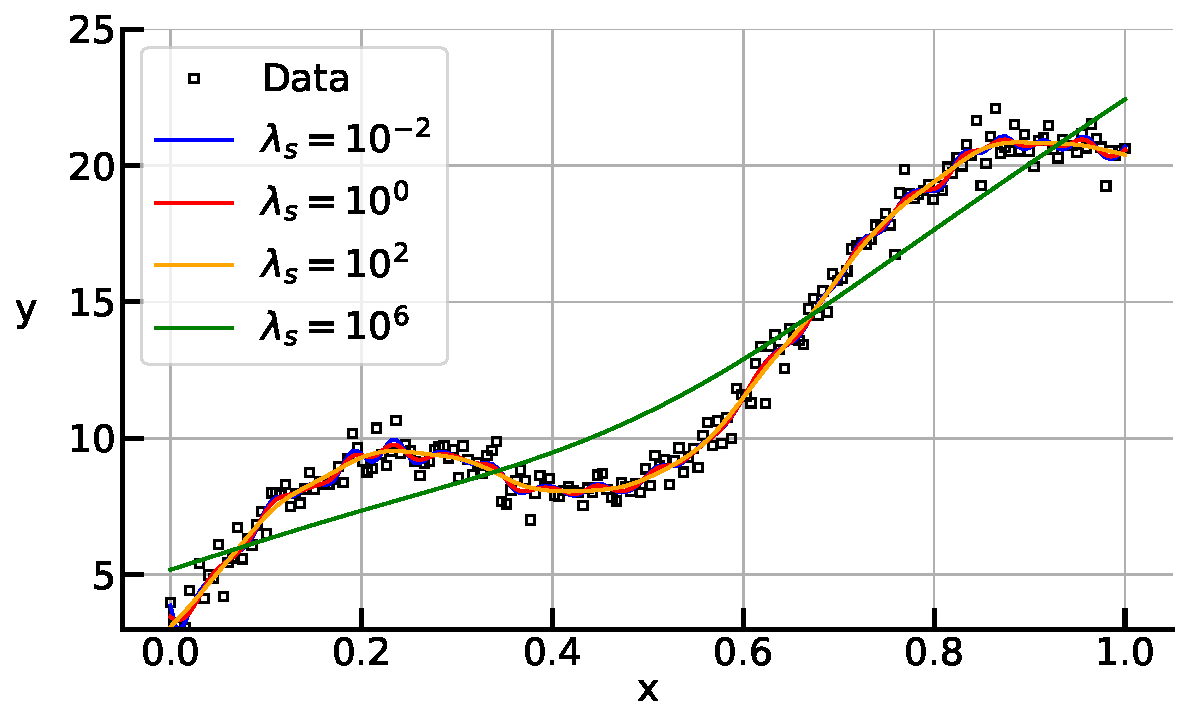
\includegraphics[width=\linewidth]{../thesisplots/p_splines.pdf}
		\caption{P-spline smooth for different $\lambda_s$}
		\label{fig:pspline}
	\end{figure}
			
	A priori knowledge can now be incorporated by an iterative approach using a sophisticated choice of the penalty matrix $D_c$ and the use of a weight matrix $V$. The scheme is depicted using the user defined constraint of monotonic increasing behavior.  
	
	Monotonic increasing behavior can be obtained using the $D_1$ matrix as penalty matrix and a diagonal weight matrix $V$, where the diagonal elements $v_j$ are given by
	
	$$v_j = \begin{cases} 0, & \quad \text{if} \ \Delta^1 \beta > 0 \\ 
						  1, & \quad \text{if} \ \Delta^1 \beta \le 0.
		 	\end{cases}$$
	
	Qualitatively, this states that the monotonic increasing penalty term is only active if adjacent coefficients $\beta_{j-1}$ and $\beta_j$ are non-increasing. An already increasing sequence of coefficients is not affected by this penalty term. \cite{hofner2011monotonicity}
	
	The penalized least squares objective function is now expanded by a term representing the user defined constraint yielding the constrained penalized least squares objective function and is given by
	
	\begin{equation} \label{PLSc}
	    Q(y; \beta) = \lVert y - X\beta \rVert^2 + \lambda_s \mathcal J_s(\beta; d) + \lambda_c \mathcal J_c(\beta; c)
	\end{equation}
	
	where $\mathcal J_c(\beta; c) = \beta^T D_c^T V D_c \beta$ using the user defined penalty matrix $D_c$ and $\lambda_c$ as parameter which determines the influence of the penalty. The parameter $\lambda_c$ is generally set quite large, i.e. $\lambda_c > 10^4$, to enforce the user defined constraint. 
	
	Again, an explicit formula for the constrained penalized least squares estimate can be given as
	
	$$\hat \beta_{PLS,c} = (X^TX + \lambda_s D_d^T D_d  + \lambda_c D_c^T V D_c)^{-1} X^T y.$$
	
	An initial estimate $\hat \beta_{init}$ is needed to compute the weight matrix. The unconstrained least squares estimate $\hat \beta_{LS}$ is a valid candidate. Now the calculation of the constrained penalized least squares estimate $\hat \beta_{PLS, c}$ and the calculation of the weight matrix $V$ is iterated until no more changes in the weight matrix $V$ appear. This scheme is called penalized iteratively-reweighted least squares and is abbreviated by \emph{PIRLS}. \cite{hofner2011monotonicity}
	
	The parameter $\lambda_c$ plays a similar role as the smoothing parameter $\lambda_s$, but should be set orders of magnitude higher than $\lambda_s$ to enforce the user defined constraint. 
	
	Figure \ref{fig:incspline} shows an example of the use of the monotonicity constraint. The smoothing parameter was set to $\lambda_s = 0.1$ and the constraint parameter was set to $\lambda_c = 6000$. For both smooths, the number of used splines $k$ was set to $30$. Visual inspection shows that the constrained, red smooth follows the a priori known behavior of monotonicity far better than the blue, unconstrained smooth.
	
	
	\begin{figure}[H]
	\centering
	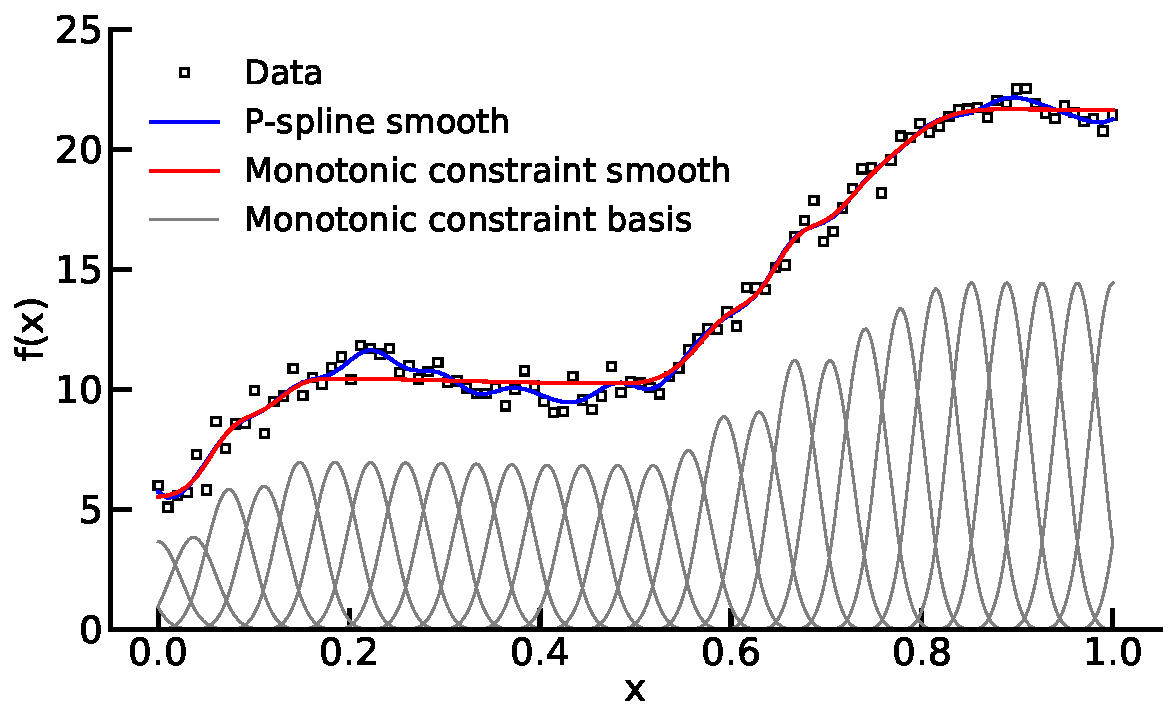
\includegraphics[width=\linewidth]{../thesisplots/inc_spline.pdf}
	\caption{Monotonicity constrained smooth}
	\label{fig:incspline}
	\end{figure}		

	This shows, that the incorporation of a priori knowledge in the fitting process using B-splines is in principle possible using a sophisticated choice of the penalty matrix $D_c$ as well as the weight matrix $V$ and an iterative fitting approach using penalized iteratively-reweighted least squares. It is important to note that this approach incorporates the a priori knowledge as soft constraints. Therefore, no guarantee can be given that the fit holds the constraint for every possible input. 

						
	\section{Penalty Matrices}
	
	
	As stated before, a priori knowledge can be introduced by the choice of the penalty matrix $D_c$ and the weight matrix $V$. It now follows a description of the different penalty matrices, which are used to enforce a priori known behavior. 
	
	
	\subsection{Monotonicity}
	
	The penalty matrix enforcing monotonic behavior is given by the use of the first order difference operator $\Delta^1$. In matrix form for $k$ splines, it is given as
	
	$$D_{monoton} = \begin{pmatrix} -1 & 1  \\ 
									& -1 & 1 \\ 
									& & \ddots & \ddots  
				    \end{pmatrix} \in \mathbb{R}^{k-1 \times k}.$$
	
	The difference between monotonic increasing and decreasing behavior is controlled by the weight matrix $V$. For increasing behavior, the weight matrix $V$ is given by the weights $v_j$ according to
	
	$$v_j = \begin{cases} 0, \quad \text{if} \ \Delta^1\beta_j > 0 \\ 
					      1, \quad \text{if} \ \Delta^1\beta_j \le 0.
			\end{cases}$$
	
	For decreasing behavior, the weight matrix $V$ is given by the weights $v_j$ according to
	
	$$v_j = \begin{cases} 0, \quad \text{if} \ \Delta^1\beta_j < 0 \\ 
						  1, \quad \text{if} \ \Delta^1\beta_j \ge 0.
			\end{cases}$$
	
	This states, that the penalty term is only applied if adjacent coefficients $\beta_{j-1}$ and $\beta_j$ are increasing or decreasing, respectively. \cite{hofner2011monotonicity} \cite{eilers2005unimodal}
	
	\subsection{Curvature}
	
	In the simplest case, the curvature of a function can either be convex or concave. The penalty matrix  enforcing this behavior is given by the use of the second order difference operator $\Delta^2$. In matrix form for $k$ splines, it is given as
	
	$$D_{curvature} = \begin{pmatrix} 1 & -2 & 1 \\ & 1 &-2 &1 \\ & & \ddots & \ddots & \ddots  \end{pmatrix} \in R^{k-2 \times k}.$$
	
	The difference between concave and convex curvature is controlled by the weight matrix $V$. For concave behavior, the weight matrix $V$ is given by the weights $v_j$ according to
	
	$$v_j = \begin{cases} 0, \quad \text{if} \ \Delta^2\beta_j < 0 \\ 1, \quad \text{if} \ \Delta^2\beta_j \ge 0. \end{cases}$$
	
	For convex curvature, the weight matrix $V$ is given by the weights $v_j$ according to
	
	$$v_j = \begin{cases} 0, \quad \text{if} \ \Delta^2\beta_j > 0 \\ 1, \quad \text{if} \ \Delta^2\beta_j \le 0. \end{cases}$$
	
	Therefore, the penalty is only applied if the second order difference of adjacent coefficients is either positive or negative, respectively. \cite{eilers2005unimodal}
	
	\subsection{Unimodality}
	
	The penalty matrix enforcing unimodal behavior can be constructed using the first order difference operator $\Delta^1$. The weight matrix $V$ now has a special structure. We assume that there is a peak in the data and therefore want to constrain the fit to include a peak. First, we need to find the index $j_{peak}$ of the spline, which has the maximal value around this  peak. The index $j_{peak}$ is now used as splitting point for the weight matrix $V$. All coefficients $j$ for $j < j_{peak}$ are constrained to be monotonic increasing, while all coefficients $j$ for $j > j_{peak}$ are constrained to be monotonic decreasing. The coefficient at position $j_{peak}$ stays unconstrained. \cite{eilers2005unimodal} The unimodal penalty matrix has the form 
	
	$$D_{unimodal} = \begin{pmatrix} -1 & 1 \\ 
									    & \ddots & \ddots  \\
									    & & 0 & 0 \\ 
									    & & & -1 & 1 \\
									    & & & &  \ddots & \ddots 
					 \end{pmatrix} \in R^{k-1 \times k}$$
	
	The weights $v_j$ have the following structure:
	
	$$v_j = \begin{cases} \begin{cases} 0, \quad \text{if} \ \Delta^1\beta_j > 0 \\ 
	1, \quad \text{if} \ \Delta^1\beta_j \le 0.\end{cases}, \quad \text{if} \ j < j_{peak} \\ \begin{cases} 0, \quad \text{if} \ \Delta^1\beta_j < 0 \\ 
	1, \quad \text{if} \ \Delta^1\beta_j \ge 0.\end{cases}  , \quad \text{if} \ j > j_{peak}  \end{cases}$$
	
	When assuming a valley in the data, the same approach as above can easily be used by multiplying the data with $-1$ or by always doing the inverse operation, i.e. finding the spline index of the valley $j_{valley}$, then constraining all splines for $j < j_{valley}$ to be monotonic decreasing and all splines for $j > j_{valley}$ to be monotonic increasing. The coefficient at position $j_{valley}$ stays unconstrained. The weights $v_j$ for the weight matrix are the given by
	
	$$v_j = \begin{cases}\begin{cases} 0, \quad \text{if} \ \Delta^1\beta_j < 0 \\ 
	1, \quad \text{if} \ \Delta^1\beta_j \ge 0.\end{cases}  , \quad \text{if} \ j < j_{valley}  \\ \begin{cases} 0, \quad \text{if} \ \Delta^1\beta_j > 0 \\ 
	1, \quad \text{if} \ \Delta^1\beta_j \le 0.\end{cases}, \quad \text{if} \ j > j_{valley} \\ \end{cases}$$
	
	\subsection{Multi-modality} 
	
	The penalty and weight matrices for the multi-modality constraint can be constructed using the scheme of unimodal constraints for each mode. It is important to find the right peak or valley points, which can be difficult with noisy data. 
	
	\subsection{Penalty Matrices for Tensor-Product Splines}
	
	The tensor-product spline basis is given by the Kronecker product of two B-spline bases, as depicted in Chapter \emph{Tensor-product splines}. To extend the framework of penalty matrices to two dimensions and tensor-product splines, we again use the concept of Kronecker products. 
	
	We want to penalized adjacent coefficient differences, but this time, in two dimensions. Therefore, an appropriate spatial neighbourhood needs to be defined. An example for such neighbourhood for the coefficient $\beta_{jk}$ is given by the coefficients left and right, i.e. $\beta_{j-1, k}$ and $\beta_{j+1, k}$, and the coefficients above and below, i.e. $\beta_{j, k-1}$ and $\beta_{j,k+1}$. 
	
	Let us now define a penalty matrix of order $d$ for each dimension and denote them by $D^1_d$ for dimension $1$ and $D^2_d$ for dimension $2$. Using the Kronecker product, we generate the expanded difference matrix $D_{d, exp}^1 = I_{d_2} \otimes D^1_d$ for $I_{d_2}$ as identity matrix of dimensions $d_2 \times d_2$ and $D_{d,exp}^2 = D^2_d \otimes I_{d_1}$ for $I_{d_1}$ as identity matrix of dimensions $d_1 \times d_1$. 
	
	Row-wise differences of order $d$ and column-wise differences of order $d$ are now obtained by applying the expanded difference matrix $D_{d,exp}^1$ and $D_{d,exp}^2$ to the coefficient vector $\beta$, respectively. 
	
	Using these concepts, in principle every possible pair of one dimensional constraints can now be constructed, e.g. unimodality in two dimensions would be obtained using the unimodal penalty matrix depicted above for each dimension. The penalty term for the constraint given by $c$ then has the form
	
	$$\mathcal J_c(\beta; c) = \beta^T D{^1_{c,exp}}^T V_1 D_{c,exp}^1 \beta + \beta^T D{^2_{c,exp}}^T V_2 D_{c,exp}^2 \beta$$
	
	with $D_{c,exp}^1 = I_{d_2} \otimes D_{unimodal}^1$ and $D_{c,exp}^2 = D_{unimodal}^2 \otimes I_{d_1}$ as individual penalty terms and $V_1$ and $V_2$ as weight matrices. The same constrained penalized least squares objective function as in Equation \ref{PLSc} can now be used to estimate the coefficients $\beta_{PLS,c}$. \cite{fahrmeir2013regression}
	
	\section{Other constraints}
	
	\subsection{Positivity}
	
	For certain physical systems, it is known a priori that the measured quantity cannot be smaller than zero. Using data-driven modeling on noisy data can lead to predictions in the interpolation and extrapolation regime which may not hold this constraint. It is therefore appropriate to use user-defined constraints for positivity.
	
	The user defined constraint for positivity again uses a weight matrix $V_{pos}$, with individual weights $v_j$ specified as follows:
	
	$$v_j = \begin{cases} 0, \quad \text{if} \ \hat y = X\hat \beta > 0\\ 1, \quad \text{if} \ \hat y = X \hat \beta \le 0 \end{cases}$$
	
	The constrained penalized least squares objective function is then of the form
	
	$$Q(y; \beta) = \lVert y - X\beta \rVert^2 + \lambda_s \mathcal J_s(\beta; d) + \lambda_{pos} \mathcal J_{pos}(\beta) $$
	
	where $\mathcal J_{pos} = \beta^T X^T V_{pos} X \beta$ is the penalty term specifying positivity and $\lambda_{pos}$ is the constraint parameter, which is set multiple orders of magnitude higher than the smoothness parameter $\lambda_s$ to enforce the constraint.
	
	Using this approach, negativity and special threshold value constraints, e.g. the output is constrained to be larger than $2$, can also be enforced.
	
	\section{Extension to Multiple Dimensions}
	
	The extension from one input to multiple inputs uses the concept of additive models given in Chapter \emph{Additive Models}. Given input data $\{ x_{i1}, \dots, x_{ip}, y_i\}$ for $i = 1, \dots, n$ and $p$ as the number of inputs, the combined model using all available B-splines and tensor-product splines is given as
	
	$$\hat y = f(x_1,..., x_p) = \sum_{i=1}^p s_i(x_i) + \sum_{i=1}^{p-1} \sum_{j>i}^p t_{i,j}(x_i, x_j) $$
	
	where $s_i(x_i)$ is the B-spline smooth given by $s_i(x_i) = X_i \beta_i$ and $t_{i, j}(x_i,x_j)$ is the tensor-product smooth given by $t_{i, j}(x_i,x_j) = X_{i,j} \beta_{i,j}$. The total number of smooths is given by $n_{smooths} = p + \frac{p(p-1)}{2}$.  Assuming the use of $k$ splines for the B-spline smooth and $k^2$ splines for the tensor-product smooth, the total number of coefficients to estimate is given by $k_{smooths} = p*k + \frac{p(p-1)}{2}k^2$. \cite{fahrmeir2013regression}
	
	Since all B-spline smooths and tensor-product spline smooths follow a linear model structure, we can combine them into one large model given by
	
	$$\hat y = X \beta$$
	
	where the combined basis matrix $X \in \mathbb{R}^{n \times k_{smooths}}$ is given by a horizontal concatenation of the individual bases and the combined coefficient vector $\beta \in \mathbb{R}^{k_{smooths}}$ is given by a vertical concatenation of the individual coefficient vectors. The combined model $\hat y_{comb}$ now has the following form
		
	$$\hat y_{comb} = X \beta = \begin{pmatrix} X_1 \dots X_p \ X_{1,2} \dots X_{p-1,p}\end{pmatrix} \begin{pmatrix} \beta_1 \\ \vdots \\ \beta_p \\ \beta_{12} \\ \vdots \\ \beta_{p-1, p}  \end{pmatrix}.$$
	
	The data term in the constrained penalized least squares objective function given in Equation \ref{PLSc} can now be evaluated using arbitrary input dimensions. 
	
	The remaining question is now how the smoothness penalty term and the constraint penalty term are constructed. For both, the concept of block diagonal matrices is applied. The smoothness penalty term $\mathcal J_s(\beta, d)$ is now given as
	
	$$\mathcal J_s(\beta; d) = \text{blockdiag}(\mathcal J_1, \dots, \mathcal J_p, J_{1,2}, \dots, \mathcal J_{p-1,p}) $$
	
	with $\mathcal J_i := \mathcal J_i(\beta_i; d_i) = \beta_i^T D_{d_i}^T D_{d_i} \beta_i$ determining the smoothness penalty term for each individual smooth $i$. $d$ is a vector, determining the order $d_i$ of the smoothness constraint for each individual smooth $i$. 
	
	The constraint penalty term $\mathcal J_c(\beta; c)$ is then given as
	
	$$\mathcal J_c(\beta; c) = \text{blockdiag}(\mathcal J_{1,c}, \dots, \mathcal J_{p,c}, \mathcal J_{1,2,c} \dots, \mathcal J_{p-1,p,c})$$
	
	with $\mathcal J_{i,c} := \mathcal J_{i,c}(\beta_i; c_i) = \beta_i^T D_{c_i}^T V_{c_i} D_{c_i} \beta_i$ determining the constraint penalty term for each individual smooth $i$ with individual weight matrix $V_{c_i}$. $c$ is a vector, determining the constraint $c_i$ for each individual smooth $i$. 
	
	The constrained penalized least squares objective function can now be written as
	
	$$Q(y; \beta) = \lVert y - X\beta \rVert^2 + \boldsymbol \lambda_s \mathcal J_s(\beta; d) + \boldsymbol \lambda_c \mathcal J_c(\beta; c) $$
	
	this time with $\boldsymbol \lambda_s, \boldsymbol \lambda_c \in \mathbb{R}^{n_{smooths}}$  defined as vectors with one value of smoothness and constraint parameter for each smooth, respectively. Using the penalized iteratively-reweighted least squares algorithm, we then obtain the estimated coefficients using the explicit solution
	
	$$\hat \beta_{PLS,c} = (X^TX + \boldsymbol \lambda_s \mathcal J_s  + \boldsymbol \lambda_c \mathcal J_c)^{-1} X^T y.$$
	
	As example, we take a look at the function 
	
	$$f(x_1, x_2) = 2\exp{\big(-\frac{(x_1 - 0.25)^2}{0.08}\big)} + x_2^2 $$
	
	for $x_1 \in [0,1]$ and $x_2 \in [0,1]$ and random Gaussian noise with $\sigma_{noise} = 0.1$. We therefore expect a peak in dimension $1$ as well as increasing behavior for dimension $2$. Using this knowledge, we create a model using the following smooths:
	
	\begin{itemize}
		\item B-spline smooth $s_1(x_1)$ using $k_{x_1} = 50$, $c = \text{peak}$, $\lambda_s = 1$ and $\lambda_c = 6000$
		\item B-spline smooth $s_2(x_2)$ using $k_{x_2} = 50$, $c = \text{inc}$, $\lambda_s = 1$ and $\lambda_c = 6000$
	\end{itemize}
		
	The fit for this model as well as the individual smooths $s_1(x_1)$ and $s_2(x_2)$ is shown in Figure \ref{fig:2d_example}. The model fits the data quite well and holds the specified constraints for the individual smooths.
		
	\begin{figure}[H]
	\centering
	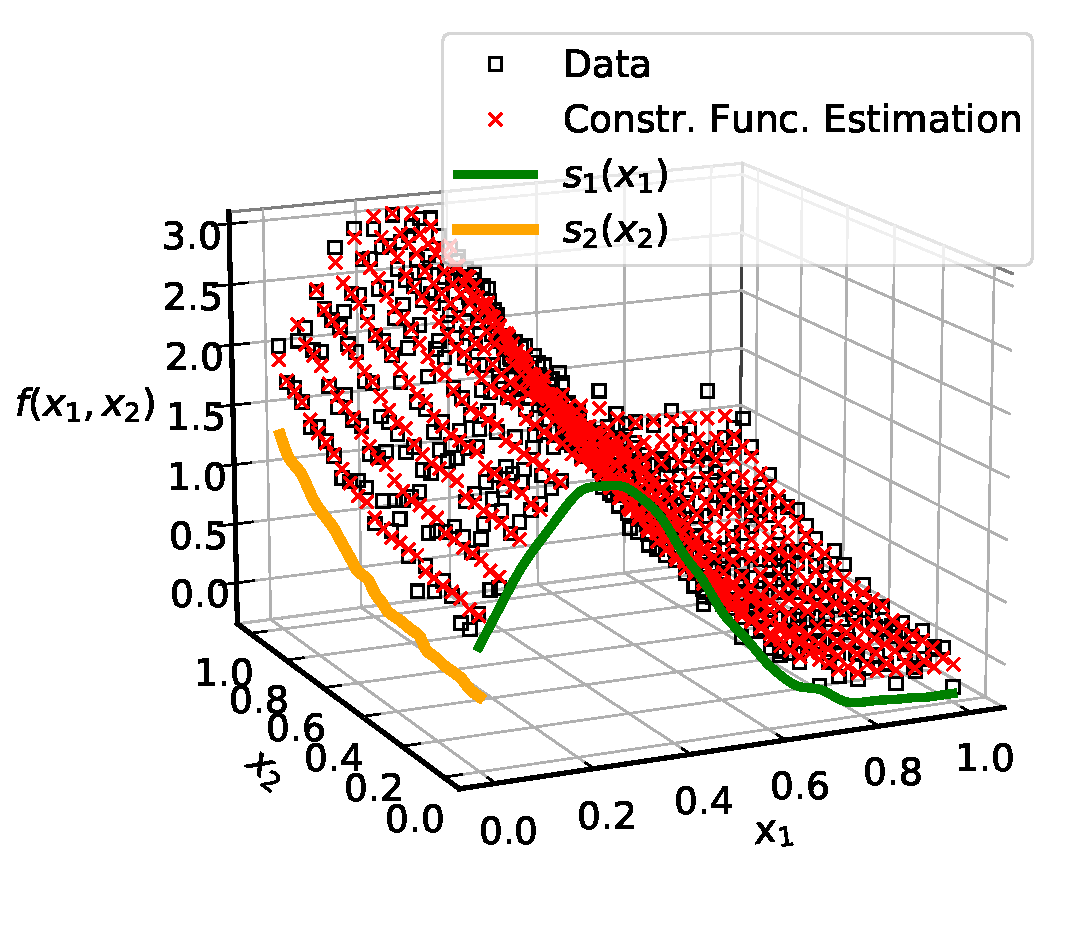
\includegraphics[width=\linewidth]{../thesisplots/2d_example.pdf}
	\caption{Test function for constrained penalized least squares fit in 2 dimension}
	\label{fig:2d_example}
	\end{figure}


	
\printbibliography
	
\end{document}